

\hypertarget{expresiones-booleanas}{%
\section{Expresiones booleanas}\label{expresiones-booleanas}}

\index{booleana, expresión} \index{expresión!booleana}
\index{lógico, operador} \index{operador!lógico}

Una \emph{expresión booleana} es aquella que puede ser verdadera
(\texttt{True}) o falsa (\texttt{False}). Los ejemplos siguientes usan
el operador \texttt{==}, que compara dos operandos y devuelve
\texttt{True} si son iguales y \texttt{False} en caso contrario:

\begin{Verbatim}[frame=single]
>>> 5 == 5
  True
>>> 5 == 6
  False
\end{Verbatim}

\texttt{True} y \texttt{False} son valores especiales que pertenecen al
tipo \texttt{bool\ (booleano)}; no son cadenas:

\index{True, valor especial} \index{False, valor especial}
\index{valor especial!True} \index{valor especial!False}
\index{booleano, tipo} \index{tipo!booleano}

\begin{Verbatim}[frame=single]
>>> type(True)
  <class 'bool'>
>>> type(False)
  <class 'bool'>
\end{Verbatim}

El operador \texttt{==} es uno de los \emph{operadores de comparación}; los demás operadores de comparación (o operadores relacionales) son:

\begin{python}[frame=single]
x != y               # x es distinto de y
x > y                # x es mayor que y
x < y                # x es menor que y
x >= y               # x es mayor o igual que y
x <= y               # x es menor o igual que y
x is y               # x es lo mismo que y
x is not y           # x no es lo mismo que y
\end{python}

A pesar de que estas operaciones probablemente te resulten familiares,
los símbolos en Python son diferentes de los símbolos matemáticos que se
usan para realizar las mismas operaciones. Un error muy común es usar
sólo un símbolo igual (\texttt{=}) en vez del símbolo de doble igualdad
(\texttt{==}). Recuerda que \texttt{=} es un operador de asignación, y
\texttt{==} es un operador de comparación. No existe algo como
\texttt{=\textless{}} o \texttt{=\textgreater{}}.

\index{comparación!operador} \index{operador!comparación}


Los operadores de comparación (o operadores relacionales) funcionan en las cadenas.  Para ver si dos cadenas son iguales:

\begin{python}[frame=single]
if palabra == 'banana':
    print('Todo bien, bananas.')
\end{python}
%
Otras operaciones relacionales son útiles para poner palabras en orden
alfabético:

\begin{python}[frame=single]
if palabra < 'banana':
    print('Tu palabra, ' + palabra + ', viene antes de banana.')
elif palabra > 'banana':
    print('Tu palabra, ' + palabra + ', viene después de banana.')
else:
    print('Todo bien, bananas.')
\end{python}
%
Python no maneja letras mayúsculas y minúsculas de la misma manera en que
lo hacen las personas. Utiliza el código ASCII para comparar letras.
ASCII es un acrónimo inglés del American 
Standard 
Code for 
Information Interchange. 
En la Figura \ref{fig:ASCII} puedes ver (parte) de los números que el código ASCII asigna a cada uno de las letras.
Podemos ver que todas las letras mayúsculas vienen antes de todas las
letras minúsculas, entonces la palabra, Piña, viene antes de banana.

\begin{Verbatim}[frame=single]
>>> "Piña" < "banana"
  True
\end{Verbatim}


\begin{figure}[t]
    \centering
    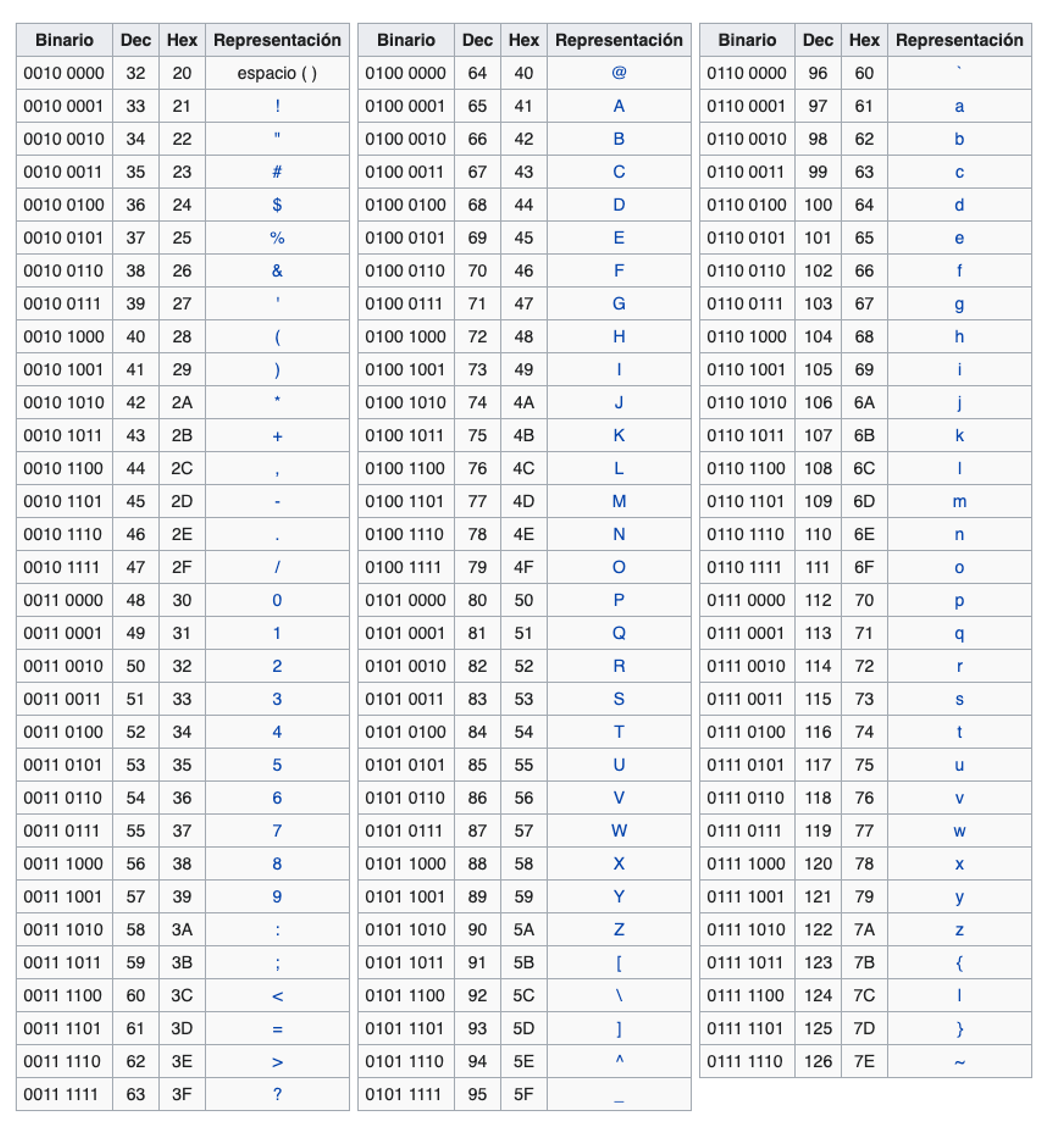
\includegraphics[width=0.85\textwidth]{images/ASCII.png}
    \caption{El código ASCII}
    \label{fig:ASCII}
\end{figure}

Python ofrece funciones \texttt{ord} y \texttt{chr} para 
averiguar el código ASCII de letras o al reves (la letra que corresponda a un código):

\begin{Verbatim}[frame=single]
>>> ord("a")
  97
>>> ord("ñ")
  241
>>> chr(97)
  'a'
\end{Verbatim}


\hypertarget{operadores-luxf3gicos}{%
\section{Operadores lógicos}\label{operadores-luxf3gicos}}

\index{lógico, operador} \index{operador!lógico}

Existen tres \emph{operadores lógicos}: \texttt{and} (y),
\texttt{or} (o), y \texttt{not} (no). El significado semántico de
estas operaciones es similar a su significado en inglés y castellano. Por ejemplo,

\texttt{x\ \textgreater{}\ 0\ and\ x\ \textless{}\ 10}

es verdadero sólo cuando \texttt{x} es mayor que 0 \emph{y} menor que
10.

\index{and, operador} \index{or, operador} \index{not, operador}
\index{operador!and} \index{operador!or} \index{operador!not}

\texttt{n\%2\ ==\ 0\ or\ n\%3\ ==\ 0} 

es verdadero si \emph{cualquiera}
de las condiciones es verdadera, es decir, si \texttt{n} es divisible por
2 \emph{o} por 3.

Finalmente, el operador \texttt{not} niega una expresión booleana, de
modo que 

\texttt{not\ (x\ >\ y)} 

es verdadero si
\texttt{x\ >\ y} es falso; es decir, si \texttt{x} es menor o igual
que \texttt{y}.

Estrictamente hablando, los operandos de los operadores lógicos deberían ser expresiones booleanas, pero Python no es muy estricto. Cualquier número distinto de cero se interpreta como 
\pythoninline{True}, i.e. verdadero.

\begin{Verbatim}[frame=single]
>>> 18 and True
  True
\end{Verbatim}

Esta flexibilidad puede ser útil, pero existen ciertas sutilezas en ese
tipo de uso que pueden resultar confusas. Es posible que prefieras
evitar usarlo de este modo hasta que estés bien seguro de lo que estás
haciendo.

\hypertarget{ejecuciuxf3n-condicional}{%
\section{Ejecución condicional}\label{ejecuciuxf3n-condicional}}

\index{condicional!sentencia} \index{sentencia!condicional}
\index{if, sentencia} \index{sentencia!if} \index{condicional!ejecución}

Para poder escribir programas útiles, casi siempre vamos a necesitar la
capacidad de comprobar condiciones y cambiar el comportamiento del
programa de acuerdo a ellas. Las \texttt{instrucciones\ condicionales}
(o simplemente los \texttt{if-then} o \texttt{if-elif-else}) nos proporciona esa capacidad. La forma más
sencilla es la sentencia \texttt{if}:

\begin{python}[frame=single]
if x > 0 :
    print('x es positivo')
\end{python}

La expresión booleana después de la \texttt{if} recibe el nombre de
\emph{condición} y se finaliza con un colon (:) y la(s) línea(s) que van
debajo de la sentencia \texttt{if} van indentadas\footnote{el término
  correcto en español sería ``sangradas'', pero en el mundillo de la
  programación se suele decir que las líneas van ``indentadas'' (Nota
  del trad.)} (es decir, llevan una tabulación o varios espacios en
blanco al principio).

\begin{figure}[t]
\centering
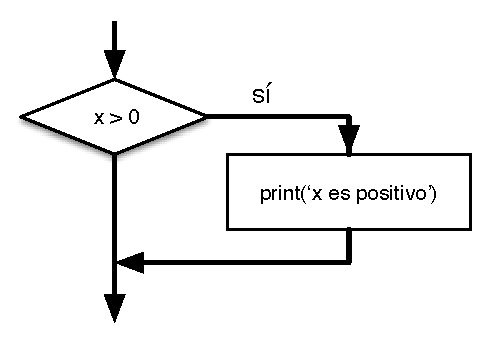
\includegraphics{images/if.eps}
\caption{If Logic}
\label{fig:if}
\end{figure}

Si la condición lógica es verdadera, la sentencia indentada será
ejecutada. Si la condición es falsa, la sentencia indentada será
omitida.

\index{condición} \index{compuesta, instrucción}
\index{instrucción!compuesta}

La instrucción \texttt{if} tiene la misma estructura que la definición
de funciones o los bucles \texttt{for}\footnote{Estudiaremos las
  funciones y los bucles en temas siguientes.}. La
instrucción consiste en una línea de encabezado que termina con el
carácter colon (:) seguido por un bloque indentado. Las instrucciones de
este tipo reciben el nombre de \emph{instrucciones compuestas}, porque
se extienden a lo largo de varias líneas.

No hay límite en el número de instrucción que pueden aparecer en el
cuerpo, pero debe haber al menos una. Ocasionalmente, puede resultar
útil tener un cuerpo sin instrucciones (normalmente como emplazamiento
reservado para código que no se ha escrito aún). En ese caso, se puede
usar la instrucción \texttt{pass}, que no hace nada.

\index{pass, sentencia} \index{sentencia!pass}

\begin{python}[frame=single]
if x < 0 :
    pass          # ¡necesito gestionar los valores negativos!
\end{python}

Si introduces una sentencia \texttt{if} en modo interactivo en la consola Python, el
prompt cambiará su aspecto habitual por puntos suspensivos (\emph{\ldots{}}), para informarte
que estás en medio de un bloque de instrucciones, como se muestra a
continuación:


\begin{Verbatim}[frame=single]
>>> x = 3
>>> if x < 10:
...    print('Pequeño')
...
  Pequeño
\end{Verbatim}

Al usar el intérprete de Python, debe dejar una línea en blanco al final
de un bloque, de lo contrario Python devolverá un error:

\begin{Verbatim}[frame=single]
>>> x = 3
>>> if x < 10:
...    print('Pequeño')
... print('Hecho')
  File "<stdin>", line 3
    print('Hecho')
        ^
SyntaxError: invalid syntax
\end{Verbatim}

No es necesaria una línea en blanco al final de un bloque de
instrucciones al escribir y ejecutar un script, pero puede mejorar la
legibilidad de su código.

\hypertarget{ejecuciuxf3n-alternativa}{%
\section{Ejecución alternativa}\label{ejecuciuxf3n-alternativa}}

\index{ejecución alternativa} \index{else, palabra clave}
\index{palabra clave!else}

La segunda forma de la instrucción \texttt{if} es la \emph{ejecución
alternativa}, en la cual existen dos posibilidades y la condición
determina cual de ellas será ejecutada. La sintaxis es similar a ésta:

\begin{python}[frame=single]
if x%2 == 0 :
    print('x es par')
else :
    print('x es impar')
\end{python}

Si al dividir \texttt{x} por 2 obtenemos como resto 0, entonces sabemos
que \texttt{x} es par, y el programa muestra un mensaje a tal efecto. Si
esa condición es falsa, se ejecuta el segundo conjunto de instrucciones.

\begin{figure}[t]
\centering
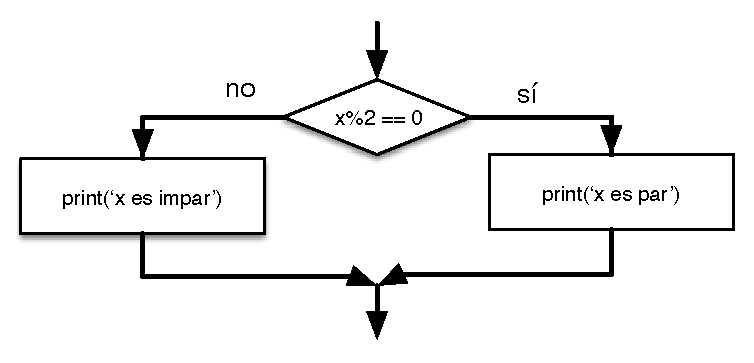
\includegraphics{images/if-else.eps}
\caption{If-Then-Else Logic}
\label{fig:if-else}
\end{figure}

Dado que la condición debe ser obligatoriamente verdadera o falsa,
solamente una de las alternativas será ejecutada. Las alternativas
reciben el nombre de \emph{ramas}, dado que se trata de ramificaciones
en el flujo de la ejecución.

\index{rama}

\hypertarget{condicionales-multiples-elif}{%
\section{Condicionales multiples
(elif)}\label{condicionales-multiples-elif}}

\index{encadenado, condicional} \index{condicional!encadenado}

Algunas veces hay más de dos posibilidades, de modo que necesitamos más
de dos ramas. Una forma de expresar una operación como ésa es usar un
\emph{condicional encadenado}:

\begin{python}[frame=single]
if x < y:
    print('x es menor que y')
elif x > y:
    print('x es mayor que y')
else:
    print('x e y son iguales')
\end{python}

\texttt{elif} es una abreviatura para ``else if''. En este caso también
será ejecutada únicamente una de las ramas.

\begin{figure}[t]
\centering
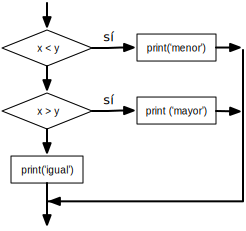
\includegraphics{images/elif}
\caption{If-Then-ElseIf Logic}
\label{fig_elif}
\end{figure}

No hay un límite para el número de \texttt{elif}. Si hay una clausula
\texttt{else}, debe ir al final, pero tampoco es obligatorio que ésta
exista.

\index{elif, palabra clave} \index{palabra clave!elif}

\begin{python}[frame=single]
if choice == 'a':
    print('Respuesta incorrecta')
elif choice == 'b':
    print('Respuesta correcta')
elif choice == 'c':
    print('Casi, pero no es correcto')
\end{python}

Cada condición es comprobada en orden. Si la primera es falsa, se
comprueba la siguiente y así con las demás. Si una de ellas es
verdadera, se ejecuta la rama correspondiente, y la instrucción termina.
Incluso si hay más de una condición que sea verdadera, sólo se ejecuta
la primera que se encuentra.

\hypertarget{condicionales-anidados}{%
\section{Condicionales anidados}\label{condicionales-anidados}}

\index{anidado, condicional} \index{condicional!anidado}

Un condicional puede también estar anidado dentro de otro. Podríamos
haber escrito el ejemplo anterior de las tres ramas de este modo:

\begin{python}[frame=single]
if x == y:
    print('x e y son iguales')
else:
    if x < y:
        print('x es menor que y')
    else:
        print('x es mayor que y')
\end{python}

El condicional exterior contiene dos ramas. La primera rama ejecuta una
sentencia simple. La segunda contiene otra sentencia \texttt{if}, que
tiene a su vez sus propias dos ramas. Esas dos ramas son ambas
instrucciones simples, pero podrían haber sido sentencias condicionales
también.

\begin{figure}[t]
\centering
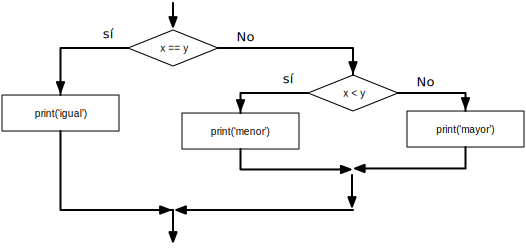
\includegraphics[width=\textwidth]{images/nested}
\caption{Nested If Statements}
\label{fig:nested}
\end{figure}

A pesar de que el indentado de las instrucciones hace que la estructura
esté clara, los \emph{condicionales anidados} pueden volverse difíciles
de leer rápidamente. En general, es buena idea evitarlos si se puede.
raw Los operadores lógicos a menudo proporcionan un modo de simplificar
las instrucciones condicionales anidadas. Por ejemplo, el código
siguiente puede ser reescrito usando un único condicional:

\begin{python}[frame=single]
if 0 < x:
    if x < 10:
        print('x es un numero positivo con un solo digito.')
\end{python}

La instrucción \texttt{print} se ejecuta solamente si se cumplen las dos
condiciones anteriores, así que en realidad podemos conseguir el mismo
efecto con el operador \texttt{and}:

\begin{python}[frame=single]
if 0 < x and x < 10:
    print('x es un numero positivo con un solo digito.')
\end{python}

\hypertarget{captura-de-excepciones-usando-try-y-except}{%
\section{Captura de excepciones usando try y
except}\label{captura-de-excepciones-usando-try-y-except}}

Anteriormente vimos un fragmento de código donde usábamos las funciones
\texttt{input} e \texttt{int} para leer y analizar un número entero
introducido por el usuario. También vimos lo poco seguro que podía
llegar a resultar hacer algo así:

\begin{Verbatim}[frame=single]
>>> velocidad = int(input("Dame un numero: "))
Dame un numero: r
Traceback (most recent call last):
  File "<pyshell>", line 1, in <module>
ValueError: invalid literal for int() with base 10: 'r'
\end{Verbatim}

Cuando estamos trabajando con el intérprete de Python, tras el error
simplemente nos aparece de nuevo el prompt, así que pensamos ``¡epa, me
he equivocado!'', y continuamos con la siguiente instrucción.

Sin embargo, si se escribe ese código en un script de Python y se
produce el error, el script se detendrá inmediatamente, y mostrará un
``traceback''. No ejecutará la siguiente instrucción.

\index{traceback}

He aquí un programa de ejemplo para convertir una temperatura desde
grados Fahrenheit a grados Celsius:

\index{fahrenheit} \index{celsius} \index{conversión de temperatura}

\begin{python}
ent = input('Introduzca la Temperatura Fahrenheit:')
fahr = float(ent)
cel = (fahr - 32.0) * 5.0 / 9.0
print(cel)
\end{python}

Si ejecutamos este código y le damos una entrada no válida, simplemente
fallará con un mensaje de error bastante antipático:

\begin{Verbatim}[frame=single]
>>> %Run fahren.py
  Introduzca la Temperatura Fahrenheit:72
  22.2222222222
\end{Verbatim}

\begin{Verbatim}[frame=single]
>>> %Run fahren.py
  Introduzca la Temperatura Fahrenheit:fred
  Traceback (most recent call last):
  File "fahren.py", line 2, in <module>
    fahr = float(ent)
  ValueError: invalid literal for float(): fred
\end{Verbatim}

Existen estructuras de ejecución condicional dentro de Python para
manejar este tipo de errores esperados e inesperados, llamadas ``try /
except''. La idea de \texttt{try} y \texttt{except} es que si se sabe
que cierta secuencia de instrucciones puede generar un problema, sea
posible añadir ciertas instrucciones para que sean ejecutadas en caso de
error. Estas instrucciones extras (el bloque except) serán ignoradas si
no se produce ningún error.

Puedes pensar en la característica \texttt{try} y \texttt{except} de
Python como una ``póliza de seguros'' en una secuencia de instrucciones.

Se puede reescribir nuestro conversor de temperaturas de esta forma:

\begin{python}
ent = input('Introduzca la Temperatura Fahrenheit:')
try:
    fahr = float(ent)
    cel = (fahr - 32.0) * 5.0 / 9.0
    print(cel)
except:
    print('Por favor, introduzca un número')
\end{python}

Python comienza ejecutando la secuencia de instrucciones del bloque
\texttt{try}. Si todo va bien, se saltará todo el bloque \texttt{except}
y terminará. Si ocurre una excepción dentro del bloque \texttt{try},
Python saltará fuera de ese bloque y ejecutará la secuencia de
instrucciones del bloque \texttt{except}.

\begin{Verbatim}
>>> %Run fahren2.py
  Introduzca la Temperatura Fahrenheit:72
  22.2222222222
\end{Verbatim}

\begin{Verbatim}
>>> %Run fahren2.py
  Introduzca la Temperatura Fahrenheit:fred
  Por favor, introduzca un número
\end{Verbatim}

Gestionar una excepción con una sentencia \texttt{try} recibe el nombre
de \emph{capturar} una excepción. En este ejemplo, la clausula
\texttt{except} muestra un mensaje de error. En general, capturar una
excepción te da la oportunidad de corregir el problema, volverlo a
intentar o, al menos, terminar el programa con elegancia.

\hypertarget{evaluaciuxf3n-en-cortocircuito-de-expresiones-luxf3gicas}{%
\section{Evaluación en cortocircuito de expresiones
lógicas}\label{evaluaciuxf3n-en-cortocircuito-de-expresiones-luxf3gicas}}

\index{cortocircuito}

Cuando Python está procesando una expresión lógica, como
\texttt{x\ >=\ 2\ and\ (x/y)\ >\ 2}, evalúa la expresión de
izquierda a derecha. Debido a la definición de \texttt{and}, si
\texttt{x} es menor de 2, la expresión \texttt{x\ >=\ 2} resulta ser
\texttt{falsa}, de modo que la expresión completa ya va a resultar
\texttt{falsa}, independientemente de si \texttt{(x/y)\ >\ 2} se
evalúa como \texttt{verdadera} o \texttt{falsa}.

Cuando Python detecta que no se gana nada evaluando el resto de una
expresión lógica, detiene su evaluación y no realiza el cálculo del
resto de la expresión. Cuando la evaluación de una expresión lógica se
detiene debido a que ya se conoce el valor final, eso es conocido como
\emph{cortocircuitar} la evaluación (o evaluación perezosa).

A pesar de que esto pueda parecer hilar demasiado fino, el
funcionamiento en cortocircuito nos descubre una ingeniosa técnica
conocida como \emph{patrón guardián}. Examina la siguiente instrucción
de código en el intérprete de Python:

\begin{Verbatim}[frame=single]
>>> x = 6
>>> y = 2
>>> x >= 2 and (x/y) > 2
  True
>>> x = 1
>>> y = 0
>>> x >= 2 and (x/y) > 2
  False
>>> x = 6
>>> y = 0
>>> x >= 2 and (x/y) > 2
  Traceback (most recent call last):
    File "<stdin>", line 1, in <module>
  ZeroDivisionError: division by zero
\end{Verbatim}

La tercera operación ha fallado porque Python intentó evaluar
\texttt{(x/y)} e \texttt{y} era cero, lo cual provoca un runtime error
(error en tiempo de ejecución). Pero el segundo ejemplo \emph{no} falló,
porque la primera parte de la expresión \texttt{x\ >=\ 2} fue
evaluada como \texttt{falsa}, así que \texttt{(x/y)} no llegó a
ejecutarse debido a la regla del \emph{cortocircuito}, y no se produjo
ningún error.

Es posible construir las expresiones lógicas colocando estratégicamente
una evaluación como \emph{guardián} justo antes de la evaluación que
podría causar un error, como se muestra a continuación:

\begin{Verbatim}[frame=single]
>>> x = 1
>>> y = 0
>>> x >= 2 and y != 0 and (x/y) > 2
  False
>>> x = 6
>>> y = 0
>>> x >= 2 and y != 0 and (x/y) > 2
  False
>>> x >= 2 and (x/y) > 2 and y != 0
  Traceback (most recent call last):
    File "<stdin>", line 1, in <module>
  ZeroDivisionError: division by zero
\end{Verbatim}

En la primera expresión lógica, \texttt{x\ >=\ 2} es \texttt{falsa},
así que la evaluación se detiene en el \texttt{and}. En la segunda
expresión lógica, \texttt{x\ >=\ 2} es \texttt{verdadera}, pero
\texttt{y\ !=\ 0} es \texttt{falsa}, de modo que nunca se alcanza
\texttt{(x/y)}.

En la tercera expresión lógica, el \texttt{y\ !=\ 0} va \emph{después}
del cálculo de \texttt{(x/y)}, de modo que la expresión falla con un
error.

En la segunda expresión, se dice que \texttt{y\ !=\ 0} actúa como
\emph{guardián} para garantizar que sólo se ejecute \texttt{(x/y)} en el
caso de que \texttt{y} no sea cero.



\hypertarget{depuraciuxf3n}{%
\section{Depuración}\label{depuraciuxf3n}}

\index{depuración} \index{traceback}

Los ``traceback'' que Python muestra cuando se produce un error
contienen un montón de información, pero pueden resultar abrumadores.
Las partes más útiles normalmente son:

\begin{itemize}
\item
  Qué tipo de error se ha producido, y
\item
  Dónde ha ocurrido.
\end{itemize}

Los errores de sintaxis (syntax errors), normalmente son fáciles de
localizar, pero a veces tienen trampa. Los errores debido a espacios en
blanco pueden ser complicados, ya que los espacios y las tabulaciones
son invisibles, y solemos ignorarlos.

\index{espacio en blanco}

\begin{Verbatim}[frame=single]
>>> x = 5
>>>  y = 6
  File "<stdin>", line 1
    y = 6
    ^
IndentationError: unexpected indent
\end{Verbatim}

En este ejemplo, el problema es que la segunda línea está indentada por
un espacio. Pero el mensaje de error apunta a \texttt{y}, lo cual
resulta engañoso. En general, los mensajes de error indican dónde se ha
descubierto el problema, pero el error real podría estar en el código
previo, a veces en alguna línea anterior.

En general, los mensajes de error te dicen dónde se ha descubierto el
problema, pero a menudo no es ahí exactamente donde se ha producido.

\hypertarget{glosario}{%
\section{Glosario}\label{glosario}}

\begin{description}
\item[condición]
La expresión booleana en una sentencia condicional que determina qué
rama será ejecutada.
\end{description}

\index{condición}

\begin{description}
\item[condicional anidado]
Una sentencia condicional que aparece en una de las ramas de otra
sentencia condicional.
\end{description}

\index{anidado, condicional} \index{condicional!anidado}

\begin{description}
\item[condicional encadenado]
Una sentencia condicional con una serie de ramas alternativas.
\end{description}

\index{encadenado, condicional} \index{condicional!encadenado}

\begin{description}
\item[cortocircuito]
Cuando Python va evaluando una expresión lógica por tramos y detiene el
proceso de evaluación debido a que ya conoce el valor final que va a
tener el resultado sin necesidad de evaluar el resto de la expresión.
\end{description}

\index{cortocircuito}

\begin{description}
\item[cuerpo]
La secuencia de sentencias en el interior de una sentencia compuesta.
\end{description}

\index{cuerpo}

\begin{description}
\item[expresión booleana]
Un expresión cuyo valor puede ser o bien \texttt{Verdadero} o bien
\texttt{Falso}.
\end{description}

\index{booleana, expresión} \index{expresión!booleana}

\begin{description}
\item[operadores de comparación]
Uno de los operadores que se utiliza para comparar dos operandos:
\texttt{==}, \texttt{!=}, \texttt{\textgreater{}}, \texttt{\textless{}},
\texttt{\textgreater{}=}, y \texttt{\textless{}=}.
\item[operador lógico]
Uno de los operadores que se combinan en las expresiones booleanas:
\texttt{and}, \texttt{or}, y \texttt{not}.
\item[patrón guardián]
Cuando construimos una expresión lógica con comparaciones adicionales
para aprovecharnos del funcionamiento en cortocircuito.
\end{description}

\index{guardián, patrón} \index{patrón!guardián}

\begin{description}
\item[rama]
Una de las secuencias alternativas de sentencias en una sentencia
condicional.
\end{description}

\index{rama}

\begin{description}
\item[instrucción compuesta]
Una instrucción que consiste en un encabezado y un cuerpo. El encabezado
termina con dos-puntos (:). El cuerpo está indentado con relación al
encabezado.
\end{description}

\index{compuesta, sentencia} \index{sentencia!compuesta}

\begin{description}
\item[instrucción condicional]
Una instrucción que controla el flujo de ejecución, dependiendo de
cierta condición.
\end{description}

\index{condicional!instrucción} \index{instrucción!condicional}

\begin{description}
\item[traceback]
Una lista de las funciones que se están ejecutando, que se muestra en
pantalla cuando se produce una excepción.
\end{description}

\index{traceback}


